\section{Diário de Bordo}

O acompanhamento das atividades do semestre foi feito com um quadro Kanban no GitHub Projects, disponível em \url{https://github.com/orgs/conloq/projects/2}. Cada tarefa é uma \textit{issue} que percorre as colunas Backlog, Ready, In progress, In review, Test e Done, com a sprint, a prioridade, o tamanho e os \textit{story points} registrados no próprio cartão. A Figura~\ref{fig:kanban} mostra o quadro na reta final do semestre.

\begin{figure}[H]
\centering
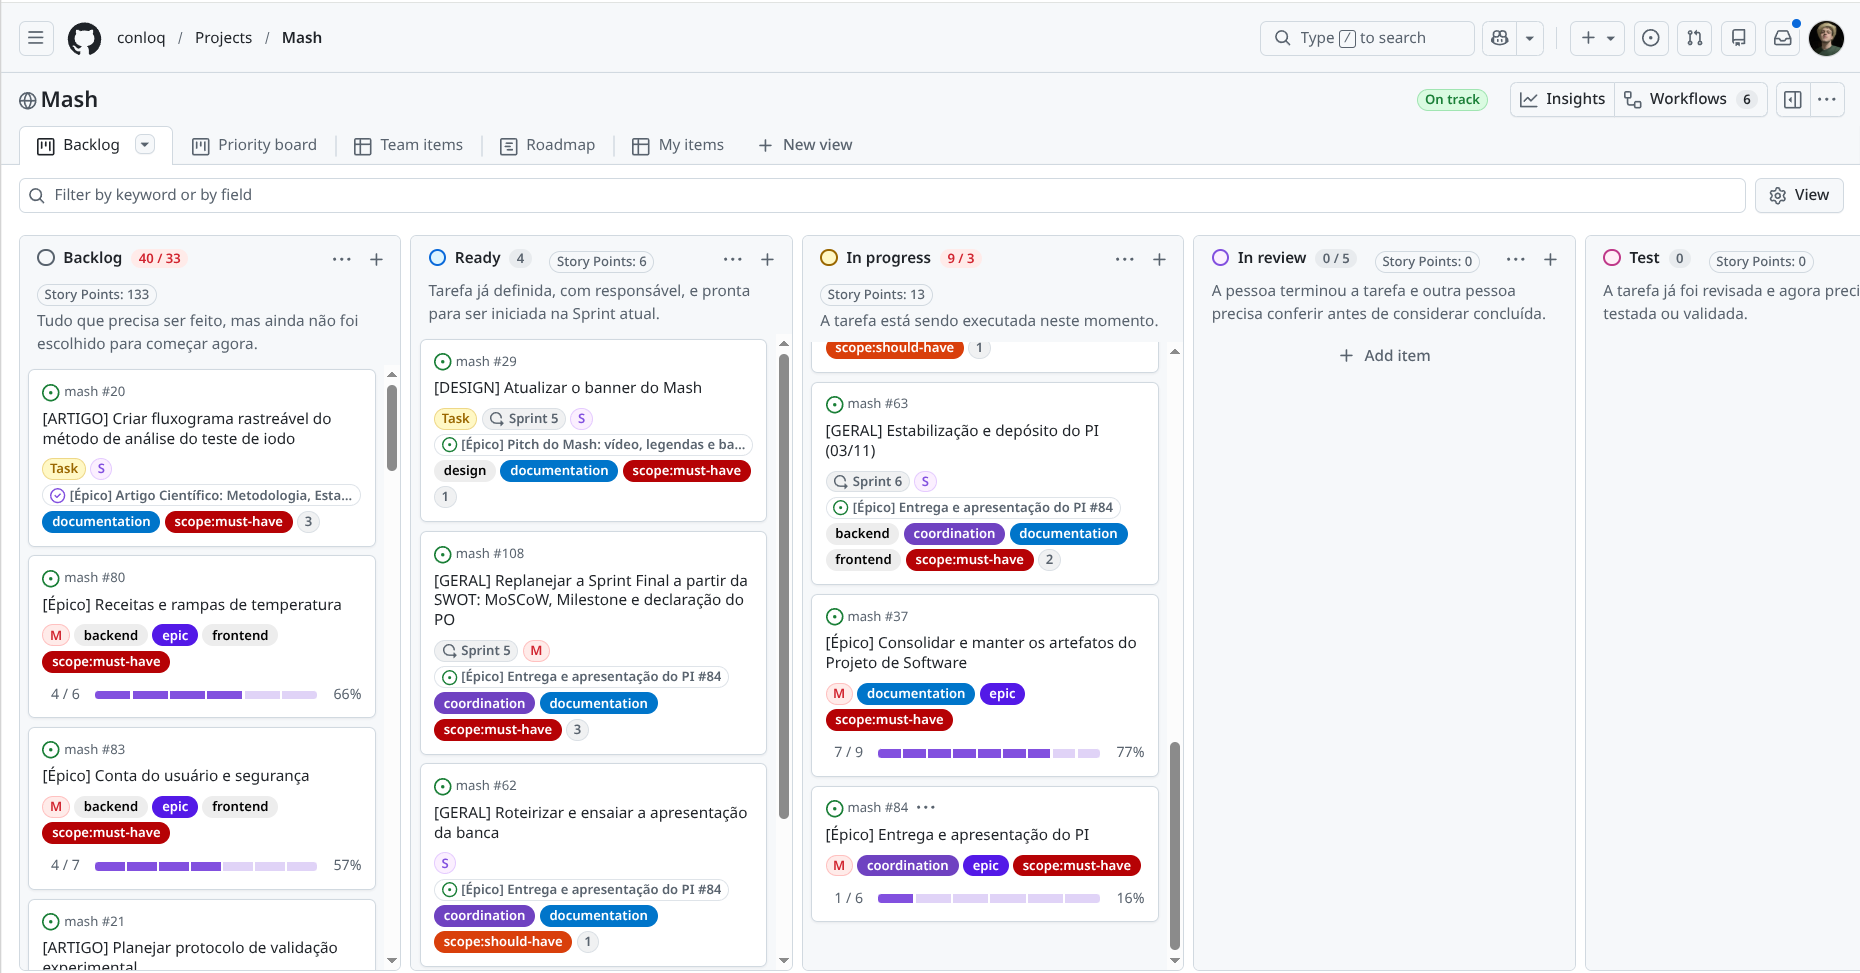
\includegraphics[width=\textwidth]{imgs/kanban.png}
\caption{Quadro Kanban do projeto no GitHub Projects}
\label{fig:kanban}
\end{figure}

O registro das atividades de cada sprint é gerado a partir dos \textit{commits} e das \textit{issues} dos repositórios da equipe e fica publicado em \url{https://github.com/conloq/logbook-backup/tree/main/diario-de-bordo}, com um arquivo por período.
